\documentclass{egpubl}
\usepackage{sbim2010}

\WsSubmission    % 
% \WsPaper       % uncomment for final version

 \electronicVersion

\ifpdf \usepackage[pdftex]{graphicx} \pdfcompresslevel=9
\else \usepackage[dvips]{graphicx} \fi

\PrintedOrElectronic

\usepackage{t1enc,dfadobe}

\usepackage{egweblnk}
\usepackage{cite}
\usepackage{subfigure}

\title[Transient Mode Techniques]
      {Transient Mode Interaction Techniques for Sketch-Based Interfaces}

% Leave blank during submission
\author[Anon]
       {Anon$^{1}$ \\
         $^1$Mysterious University\\
       }

\begin{document}

\maketitle

\begin{abstract}

This paper describes an exploration of transient mode interaction
methods suitable for use in sketch-based interfaces. Each technique is
triggered by a sketched gesture that invokes a transient mode change,
enabling users to seamlessly transition between drawing, forming
selections, and issuing commands. These techniques are demonstrated in
a simple cartoon sketching program called SKRUI Draw. Three idioms are
described: flow selection, scribble-fill, and structural ink. While
SKRUI Draw remains an experimental system, the sketch-based
interaction techniques it provides show promise.

\begin{classification} % according to http://www.acm.org/class/1998/
\CCScat{Computer Graphics}{I.3.6}{Interaction Techniques}
\end{classification}

\end{abstract}

%-------------------------------------------------------------------------
\section{Introduction}

Sketch-based applications are often used to support visual thinking
and informal reasoning. It is important to support these activities
without needlessly imposing structure. Typically, software tools
present functions using persistent modes, such as pencil mode, fill
mode, select mode, and so on. To perform an action, users temporarily
shift focus to the editing controls to find and activate the
appropriate widget before returning to work.

This paper presents several mode switching techniques that address the
problem of persistent mode. The techniques are \emph{transient}
because input reverts back to the default sketching mode when it is no
longer needed. Each transient technique is triggered by interpreting
sketched gestures.

This work presents three techniques: flow selection, scribble-fill,
and structured ink. They are implemented in a simple cartoon drawing
environment called SKRUI Draw (shown in Figure~\ref{fig:skrui-draw}).

\begin{figure}[htb]
  \label{fig:skrui-draw}
  \centering
  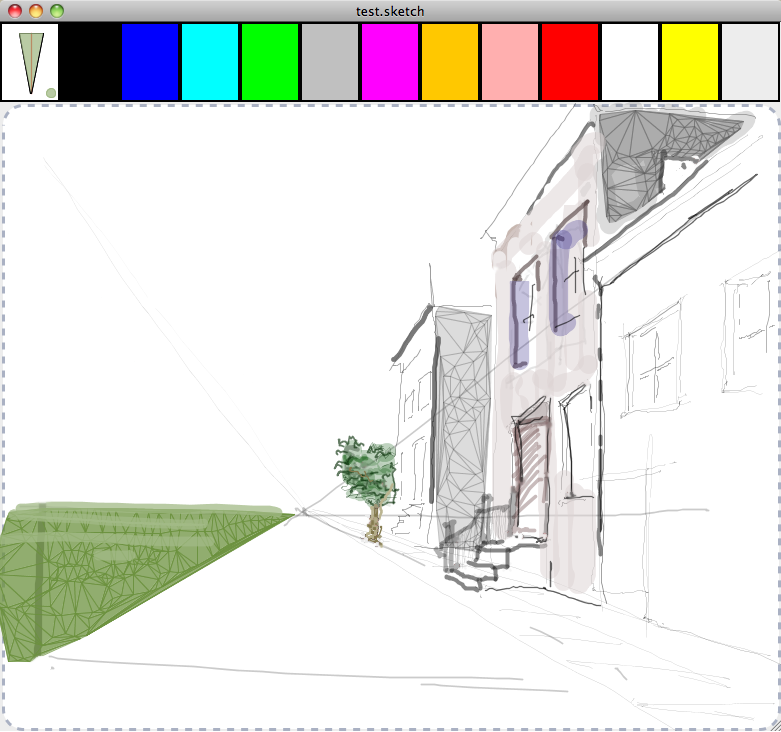
\includegraphics[width=.9\linewidth]{img/shaun.png}
  \caption{SKRUI Draw showing an architect's sketch.}
\end{figure}

\section{Related Work}

The Inferred Mode Protocol~\cite{saund-inferred-mode} provides a
framework for sketching without persistent modes. The system
interprets pen input using context to mediate user intent. When
unclear or ambiguous input is found, the system might wait for more
information, or it could ask the user to resolve the problem.

Li \textit{et. al} studied several methods for switching modes in
pen-based systems~\cite{li-mode-switching}. Four of five technique
reviewed requires special hardware: a pen barrel button, a button for
the user's non-dominant hand, pen pressure sensing, and the `eraser'
end of the pen. The last technique, a dwell gesture, requires no
additional hardware. The dwell technique was the least efficient and
least liked in their study, while the offhand button was the most
effective.

Mode-changing gestures should be `different' enough that users are
unlikely to trigger them by accident but simple enough that they can
be remembered and issued without error. Scriboli's \emph{delimiters}
provide a point of departure in this
regard~\cite{hinckley-scriboli}. The delimiters are gestures that
appear at the end of a selection stroke that people are unlikely to
make otherwise, but are easily recognized and enable users to give
commands on the selected region.

Thierjung \textit{et. al} studied methods for recognizing filled or
hatched regions by analyzing stroke
features~\cite{thierjung-hatching}. The current approach is designed
to be interactive and is recognized as the stroke is made. Thierjung's
approach is more extensible but it is not interactive.

A portion of this system extends prior work on Flow
Selection~\cite{johnson-flow-selection}. It is a method for easily
selecting and adjusting portions of a drawn stroke. A dwell gesture
causes a selection to `grow' outward from the nearest point on the
line. Each point is partially selected. The longer the dwell
continues, the more strongly each point is selected. If the user drags
the pen, points are translated some amount depending on how strongly
they are selected and how much the pen has moved.

\section{Transient Interaction Techniques}

The following sections present three experimental transient
interaction techniques, developed on the principle that \emph{the user
  should never have to set down their pen}. These techniques aim to
minimize the cognitive overhead associated with sketch-recognition
based user interfaces. Transient modes should require minimal effort
to enter and no effort to exit.

The methods are implemented in a simple cartoon sketching environment
called SKRUI Draw, written in Java 1.6. These techniques were
deliberately developed together to get a sense for how well (or not)
they work as an ensemble.

\subsection{Flow Selection}

\begin{figure}
  \centering \subfigure[Creating a hinge by selecting near the end of
    a stroke.] {
    \label{fig:fs-hinge-b} 
    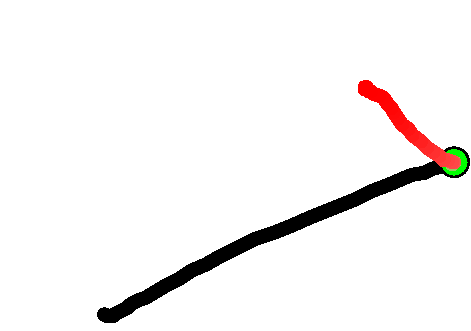
\includegraphics[width=0.42\linewidth]{img/fs-hinge-b.pdf}
  }
\hspace{0.4cm} \subfigure[The corrected stroke has been rotated and scaled.] {
    \label{fig:fs-hinge-c} 
    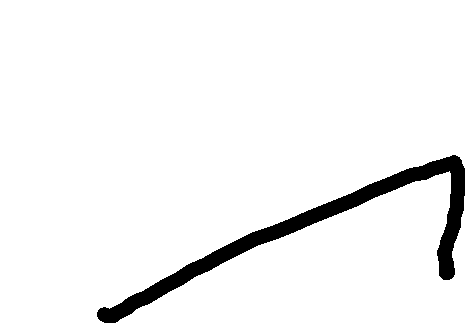
\includegraphics[width=0.42\linewidth]{img/fs-hinge-c.pdf}
  }
  \caption{Flow-selecting near the end of a stroke enables users to
    use corners as a hinge, allowing the selected portion of a stroke
    to be rotated and scaled.}
  \label{fig:fs-hinge}
\end{figure}

% - Figure of multiple-select and moving the selected strokes.

\begin{figure}
  \centering \subfigure[] {
    \label{fig:fs-multi-a} 
    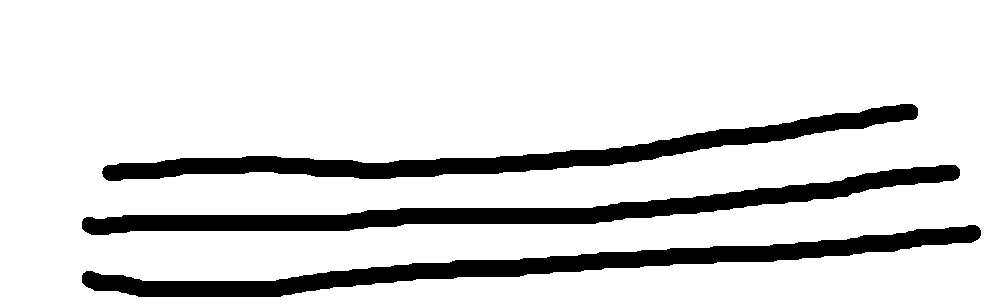
\includegraphics[width=0.3\linewidth]{img/fs-multi-a.pdf} 
  }
\subfigure[] {
    \label{fig:fs-multi-b} 
    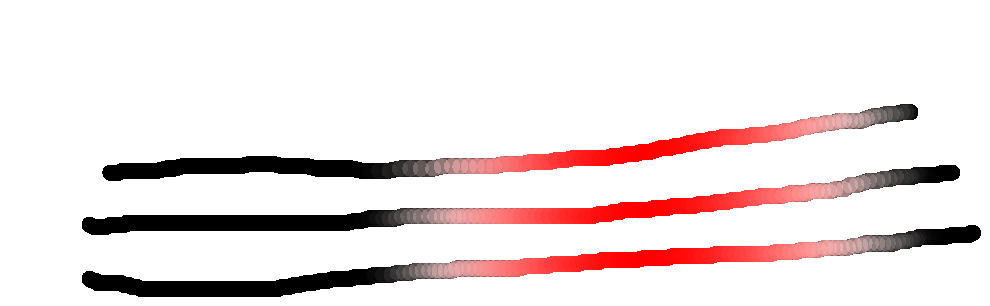
\includegraphics[width=0.3\linewidth]{img/fs-multi-b.pdf}
  }
\subfigure[] {
    \label{fig:fs-multi-c} 
    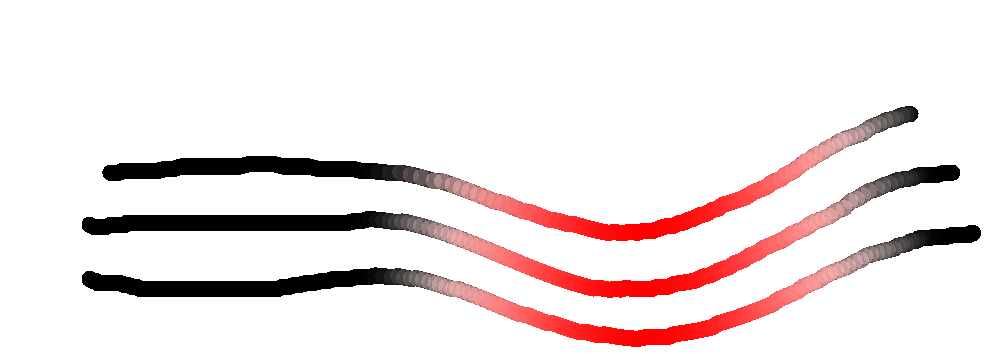
\includegraphics[width=0.3\linewidth]{img/fs-multi-c.pdf}
  }
\caption{Multiple stroke flow-selection: If the user taps the pen
  immediately before beginning a flow selection, multiple strokes are
  selected. Each tap adds a constant distance to the area of
  effect. Each stroke is equally effected by modifications.}
  \label{fig:fs-multi}
\end{figure}

\begin{figure}
  \centering \subfigure[] {
    \label{fig:fs-heat-a} 
    
\includegraphics[width=0.3\linewidth]{img/fs-heat-a.pdf} 
  }
\subfigure[] {
    \label{fig:fs-heat-b} 
    
\includegraphics[width=0.3\linewidth]{img/fs-heat-b.pdf}
  }
\subfigure[] {
    \label{fig:fs-heat-c} 
    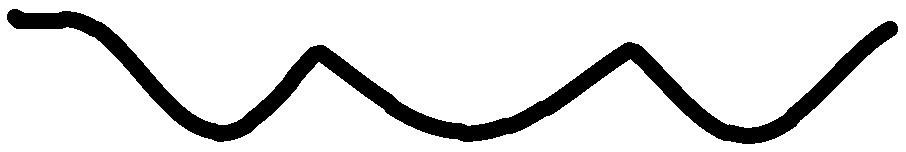
\includegraphics[width=0.3\linewidth]{img/fs-heat-c.pdf}
  }
\caption{Selecting and editing multiple regions of the same
  stroke. Panels~\ref{fig:fs-heat-a} and~\ref{fig:fs-heat-b} show the
  user making a disjoint selection of the same stroke;
  in~\ref{fig:fs-heat-c} the user manipulates the selection.}
  \label{fig:fs-heat}
\end{figure}

The current system extends prior work on Flow
Selection~\cite{johnson-flow-selection} in three ways. First, if the
user begins a flow selection near the end of a stroke, the selection
will pause momentarily when it reaches a corner. When the corner point
is 70\% selected and one neighbor is less than 35\% selected, it acts
as a hinge and is shown as a large colored dot. If the user drags the
stylus, selected points are scaled and rotated about the
hinge. Figure~\ref{fig:fs-hinge} illustrates this process. Corners are
found using the MergeCF algorithm~\cite{wolin-smr}.

Second, users can select more than one stroke by tapping before
starting the flow selection (See Figure~\ref{fig:fs-multi}). Each tap
expands the radius of influence by 30 pixels.

Last, selections persist for a short time after they are made,
enabling users to select and operate on more than one region of the
same stroke (see Figure~\ref{fig:fs-heat}). Flow selection can be
thought of as \emph{heating} a stroke; heated regions are
malleable but \emph{cool} over time until they are no longer
selected.

A point's selection strength is a product of two functions:
\emph{effort} and \emph{strength}. Effort is calculated using a
message passing scheme. Messages originate at the selection's
\emph{epicenter}---the point on the stroke that is closest to the
stylus.

Effort represents how long the user must dwell for a point to become
fully selected. In this implementation, effort is simply the
accumulated curvilinear distance from the selection epicenter to the
point in question, plus penalties imposed by intervening corners. The
effort message passing function is:
\begin{equation}
E[next] = E[i] + distance(i, next) + penalty(i)
\end{equation} 
Variables $i$ and $next$ are neighboring points of the same
stroke. The effort value for the epicenter point is defined as
zero. The penalty function returns 130 for corners, and zero for other
points.

The strength function depends on a point's effort value $E[i]$, the
dwell duration $t$, and the existing selection strength $S[i]$ from
any previous selections. An experimentally found constant, $C$, is
used to control how quickly the selection spreads (in this
implementation it is $0.1$.) The following presents the strength
function in two steps.
\begin{equation}
v[i] = \left\{
     \begin{array}{cl}
       (cos(\frac{\pi \cdot E[i]}{t \cdot C})+1) / 2 & : E[i] < t \cdot C\\
       \\
       0 & : otherwise
     \end{array}
   \right
\end{equation}
\begin{equation}
S[i] = max(v[i], S[i])
\end{equation}

Note that the updated strength value can not decrease until the
selection begins cooling, or until the user selects a different
stroke.

\subsection{Scribble Fill}

\begin{figure}
  \centering \subfigure[A scribble-like gesture causes the SKRUI Draw
    to enter a fill-mode.] {
    \label{fig:scr-a} 
    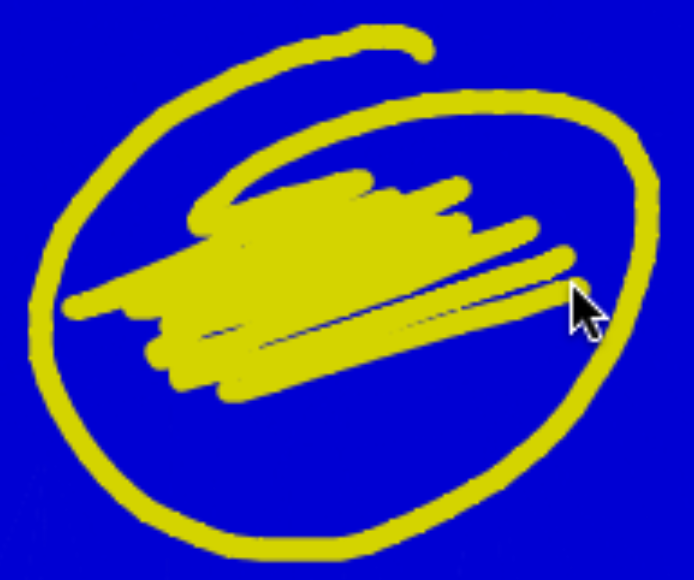
\includegraphics[width=0.42\linewidth]{img/scribble-fill-a.png}
  }
\hspace{0.4cm} \subfigure[Moments later the region is filled using the
  same pen color.] {
    \label{fig:scr-b} 
    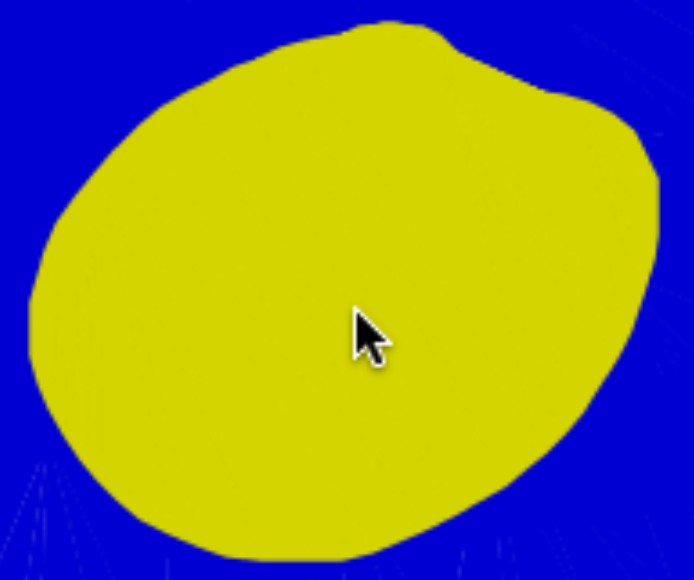
\includegraphics[width=0.42\linewidth]{img/scribble-fill-b.png}
  }
  \caption{Scribble-fill: to color a region, the user issues a
    scribble gesture, characterized by lines with very sharp corners
    between them. Once a scribble is recognized, it fills in the
    convex hull of the pen path, and continues to add points to the
    hull as the user optionally drags the stylus.}
  \label{fig:scr}
\end{figure}

People often make colored or hatched regions in a sketch. Using pencil
and paper, one way of shading a region is to scribble back and forth,
creating the visual suggestion of a shaded region. The back-and-forth
motion (illustrated in Figure~\ref{fig:scr-a}) serves as a gesture
that initiates a mode change to create a filled region.

Because the gesture must be detected as the user draws a stroke, we
can not use the MergeCF corner finding algorithm used in other parts
of SKRUI Draw. Instead, corners are resolved as the stroke
progresses. For each point, two vectors are created that extend a
constant distance outward along the pen path in both directions (in
this implementation, the distance is 10 pixels in each direction). If
the angle between these two vectors is less than 1 radian, it is a
corner candidate. Typically, this creates clusters of candidates. The
accepted corner is the one with the smallest angle in a candidate cluster.

A scribble-fill gesture is identified by a series of corners separated
by straight segments. The ink between corners is considered straight
if its ideal length (the line joining its endpoints) is no less than
90\% of its actual curvilinear path length. To trigger a
scribble-fill, the current implementation requires six consecutive
corners and line segments that satisfy these constraints. 

Once a scribble-fill gesture has been recognized, the pen path is used
to form a convex hull, which is filled using the current pen color
(shown in Figure~\ref{fig:scr-b}). Each additional pen point is added
to the hull.

Lifting the pen ends the fill operation, and the user may continue
sketching with the familiar pencil tool. However, if the next pen drag
begins in the recently created filled region, it triggers another
scribble-fill. This lets the user easily create filled regions that
are not convex.

\subsection{Structured Ink}

Designers often make conceptual drawings with marks that guide
production of important geometric properties. For example, when
drawing a cylindrical object, the designer might begin by drawing a
bounding parallelepiped to anchor production of subsequent marks. While
this part of the drawing is not strictly part of the object under
consideration, it is certainly part of the designer's thinking and
production process. Such `scaffolding lines'~\cite{company-modes}
appear in many design domains, particularly those concerning physical
form.

SKRUI Draw supports users to create scaffolding via drawn
gestures. This \emph{structured ink} allows users to place points and
lines and use them to guide production of new sketch input. They also
serve as editing controls for working with nearby elements.

A structured point is created with a drawn gesture consisting of a dot
followed by two short intersecting lines. The structured point is
created at the intersection of the two lines. The ink associated with
the gesture is removed. Structured point gestures are identified with
a constraint-based recognizer conceptually similar to
LADDER~\cite{hammond-ladder}. Additionally, the stroke components of a
gesture must be made in a particular sequence, which helps reduce
false positives.

Structured points provide visual guides. In order to remove reduce
clutter, only the three most recently created or activated points are
used to show guides. After 30 seconds, structured points are no longer
considered active. Tapping a structured point once reactivates it.

There are several types of guides. A line is drawn from the most
recent point to the current pen location. Lines connect the three most
recently active points, and their midpoints are also shown. Three
active points are used to fit a circle. Figure~\ref{fig:struct} shows
all guide types.

Structured points may be used to control nearby sketched ink by
tapping them. Two taps cause nearby lines move (see
Figure~\ref{fig:struct-b}). If a line's endpoint is near the
structured point, it is rotated and scaled to coincide with the
structured point, using the opposing endpoint as a hinge. When the
middle section of line passes near a structured point, the whole line
is translated to meet the structured point. Tapping three times will
rectify nearby ink (see Figure~\ref{fig:struct-c}).

\begin{figure}
  \centering \subfigure[Rough triangle with three nearby structured points.] {
    \label{fig:struct-a} 
    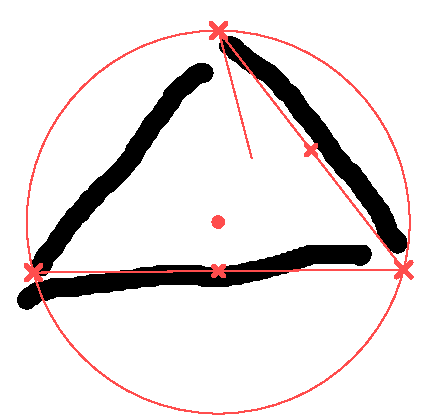
\includegraphics[width=0.27\linewidth]{img/str-a.pdf}
  }
\hspace{0.2cm} \subfigure[Two taps: Rotate and scale lines.] {
    \label{fig:struct-b} 
    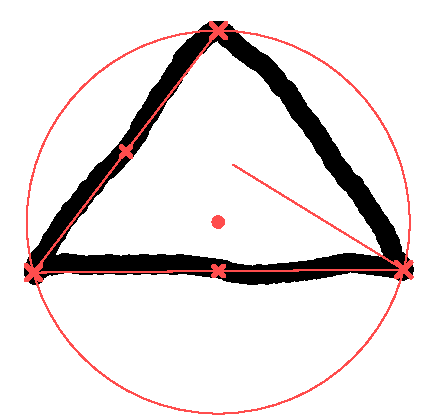
\includegraphics[width=0.27\linewidth]{img/str-b.pdf}
  }
\hspace{0.2cm} \subfigure[Three taps: Straightening lines.] {
    \label{fig:struct-c} 
    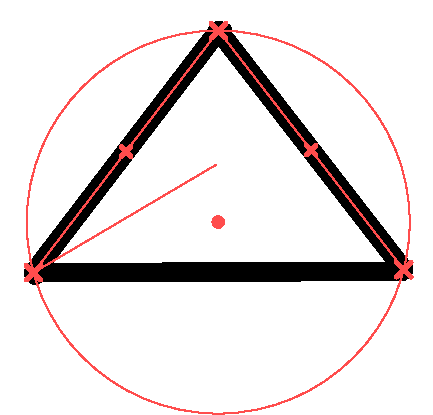
\includegraphics[width=0.27\linewidth]{img/str-c.pdf}
  }
  \caption{Structured points can serve as editing nodes. Tapping twice
    causes nearby ink to scale and rotate to end at the structured
    point. Tapping three times rectifies those same lines. The
    dangling line in each figure is the guide line connecting the pen
    location to the most recently activated point. }
  \label{fig:struct}
\end{figure}

\section{Future Work}

The mode-switching techniques described in this paper are
experimental. They will be improved and new ones will be
added. Progress will be guided in part by user testing, which will
supply feedback about recognition errors caused by different user
drawing styles and expectations, as well as preferences about which
methods feel intuitive.

Further work must be done to simplify SKRUI Draw's software
architecture to accommodate additional transient modes. Adding modes
increases user choice but complicates the system architecture. It also
increases user cognitive load: gestures must be learned and
remembered.

There are planned improvements to each technique discussed
earlier. Encircling a region and dwelling without lifting the pen (as
in Scriboli's Dwell gesture) could trigger a flow selection of the
encircled area, and enable users to perform commands on the selected
region. This affords the ability to erase and to select colors or
thickness properties from the selected area. The `heating/cooling'
metaphor might enable overtrace strokes to correct flow-selected
areas. Currently flow selection only operates on raw ink, but it
should be extended to also work on scribble-filled regions as well.

Scribble-fill could use existing elements as guides (both structured
lines and raw ink.) The filled region should then `stick' to the
existing boundaries so that changing the guide also changes the filled
region. While it is possible (and relatively easy) to create filled
regions that are not convex, it requires multiple pen strokes. A
significant improvement to scribble fill would be to generate
non-convex shapes regions based on the pen path.

It is not clear if the current method for creating structured ink is
the best way. Mechanical engineers sketching on paper draw guides
alongside lines to indicate the subject's
shape~\cite{company-modes}. These lines are differentiated by their
appearance: dashed or thin, light marks for auxiliary lines; thick,
overtraced lines for object boundaries. Given that sketch-based tools
often aim to provide a paper-like experience, it is worthwhile to
explore how structured ink might be inferred based on the visual
appearance of drawn lines.

\section{Conclusion}

This paper has presented three transient mode interaction techniques
for sketch-based design tools. While they are still experimental they
serve as objects to think with and might lead to a set of interaction
idioms suitable for sketch interaction. The Java code for this project
is open source and freely available on the Internet. I thank Shaun
Moon for testing SKRUI Draw and making the sketch in
Figure~\ref{fig:skrui-draw}.

\bibliographystyle{eg-alpha}

\bibliography{sketch-bibliography}

%-------------------------------------------------------------------------

\end{document}

% This paper was brought to you by Moon8:
% http://rainwarrior.thenoos.net/music/moon8.html
% (Dark Side of the Moon performed on an NES)

